\hspace{1cm}Gravitational waves are already used as an important member of multi-messenger astronomy and these can be used to study in depth many objects or phenomena such as:

\begin{itemize}

\item Cataclysmic variables
\item Binary Neutron Stars
\item Young Neutron Stars (the r-mode instability)
\item Low-mass X-ray binaries
\item CMB and Galaxy formation

\end{itemize}

\hspace{1cm}Gravitational waves are emitted by the masses and sent as ripples across spacetime which is completely different from the mechanism of production and transmission of EM waves. Therefore, it could give us more information on the subject matter at hand.

\hspace{1cm}Gravitational waves provide further information about black holes that would otherwise be invisible. Gravitational waves also weakly interact with matter (apart from lensing), thereby reducing energy lost or scattered before reaching the detector. This implies better understanding of inconspicuous regions of space, like the interior of a supernova or the Big Bang.

\subsection{Uses of their Detection}

\hspace{1cm} Gravitational Waves are also used in Astronomy because it allows us to observe the universe the universe in a different way, providing us information about matter such as:

\subsubsection*{Information about the Big Bang}
\hspace{1cm}Gravitational waves have travelled almost unimpeded through the universe since they were generated (which happened $10^{-24}$s after the Big Bang, far earlier than the CMB radiation). Possibilities of non-inflation mechanisms that produce gravitational waves are high. One such possibility could be cosmic strings, which ought to be detectable using gravitational waves. Observations of compact binaries in spiral made by the LIGO/VIRGO experiments can to give us a lot more information about the system than just the binary masses and spins:

\subsubsection*{Test the theory of General Relativity}
\hspace{1cm}They can be used for high-precision tests of general relativity. Radiation reaction to some scalar waves in scalar-tensor theories has a signature that can be found with high precision in LIGO/VIRGO.

\subsubsection*{Detection of the Hubble Constant}
\hspace{1cm}They can be used to measure the Universe’s Hubble constant, deceleration parameter, and cosmological constant.Gravitational waves bring a new window to validate the general theory of relativity and cosmological constant as the perfect/correct theory of gravity and the expanding universe(cosmic acceleration). Hubble's Constant shows the expansion of the Universe by showing how distant galaxies are moving away from us and is given by:
 
\begin{equation}
v = H_0 \times d
\end{equation}

where, v is the Velocity of a galaxy, in $kms^{-1}$

      $H_{0}$ is the Hubble Constant, measured in $kms^{-1}Mpc^{-1}$
      
      d is the distance of the galaxy from the earth in megaparsecs(Mpc)

\vspace{1cm}

\begin{figure}[h]
    \centering
    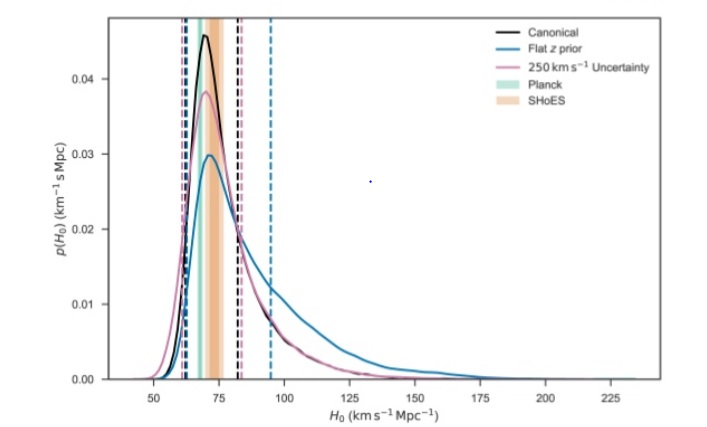
\includegraphics[scale=0.9]{images.tex/HCGW.jpg}
    \caption{Hubble's Constant using Gravitational waves.\\
    Source :- \href{https://www.researchgate.net/profile/Michael-Ross-9/publication/324600496}{A gravitational-wave standard siren measurement of the Hubble constant, Pg 3}}
\end{figure}

\subsubsection*{Polarization of Gravitational Waves}
\hspace{1cm}Gravitational waves carry 2 independent polarizations. A wave will usually have a combination of both. Some sources (rotating) will emit both polarizations with some lag between them. Studying this would give the nature of the source and its rotation.


\subsubsection*{Centrifuge of Binary Stars}
\hspace{1cm}A more careful calculation shows that, for unequal masses, the quadrupole amplitude and the rate of shrinking depend on the masses only through the combination:
\begin{equation}
\ M=\mu^{3/5} \times M^{2/5}\
\end{equation}
\hspace{1cm}This is called the chirp mass, where, $\mu$ is the reduced mass and M the total mass. The chirp mass can be easily determined if the shrinking time is observed in gravitational radiation. After measuring the amplitude, the only quantity that would not be known to us is the radial distance r from here to the source. By observing the gravitational waves that are produced by shrinking orbits due to loss in energy via gravitational radiation, we can thus obtain the distance to the source. This is another example how gravitational wave observations provide information that is hard to find using electromagnetic waves.

\subsubsection*{Spiralling of Black Holes and Neutron Stars}
\hspace{1cm}For a Neutron star or black hole spiralling inwards, the inward spiral has a sort of “map” of it that are emitted in the form of gravitational waves. Analysis of these waves could give information of the body, help determine the type of body(black hole or any other exotic object like a naked singularity)  and can be studied better by LISA for low masses and high frequencies as opposed to LIGO/VIRGO that can capture large masses and low frequencies.


\subsubsection*{Inference from uses of GW}

\hspace{1cm}In summary, we can say gravitational waves provide a new tool for astronomy as well as cosmology and will be ever evolving in terms of types of observations possible ranging from new ways to test for dark matter and the validity general relativity with high precision and observations that simply would not be possible with just electromagnetic waves.This also provides an alternate method to validate the cosmological constant, Hubble’s constant, and various other uses. This section was referred from these 2 papers \cite{Schutz_1999},\cite{Mukherjee_2020}

\pagebreak
